\documentclass[journal, a4paper]{IEEEtran}

% some very useful LaTeX packages include:

%\usepackage{cite}      % Written by Donald Arseneau
                        % V1.6 and later of IEEEtran pre-defines the format
                        % of the cite.sty package \cite{} output to follow
                        % that of IEEE. Loading the cite package will
                        % result in citation numbers being automatically
                        % sorted and properly "ranged". i.e.,
                        % [1], [9], [2], [7], [5], [6]
                        % (without using cite.sty)
                        % will become:
                        % [1], [2], [5]--[7], [9] (using cite.sty)
                        % cite.sty's \cite will automatically add leading
                        % space, if needed. Use cite.sty's noadjust option
                        % (cite.sty V3.8 and later) if you want to turn this
                        % off. cite.sty is already installed on most LaTeX
                        % systems. The latest version can be obtained at:
                        % http://www.ctan.org/tex-archive/macros/latex/contrib/supported/cite/

\usepackage{graphicx}   % Written by David Carlisle and Sebastian Rahtz
                        % Required if you want graphics, photos, etc.
                        % graphicx.sty is already installed on most LaTeX
                        % systems. The latest version and documentation can
                        % be obtained at:
                        % http://www.ctan.org/tex-archive/macros/latex/required/graphics/
                        % Another good source of documentation is "Using
                        % Imported Graphics in LaTeX2e" by Keith Reckdahl
                        % which can be found as esplatex.ps and epslatex.pdf
                        % at: http://www.ctan.org/tex-archive/info/

%\usepackage{psfrag}    % Written by Craig Barratt, Michael C. Grant,
                        % and David Carlisle
                        % This package allows you to substitute LaTeX
                        % commands for text in imported EPS graphic files.
                        % In this way, LaTeX symbols can be placed into
                        % graphics that have been generated by other
                        % applications. You must use latex->dvips->ps2pdf
                        % workflow (not direct pdf output from pdflatex) if
                        % you wish to use this capability because it works
                        % via some PostScript tricks. Alternatively, the
                        % graphics could be processed as separate files via
                        % psfrag and dvips, then converted to PDF for
                        % inclusion in the main file which uses pdflatex.
                        % Docs are in "The PSfrag System" by Michael C. Grant
                        % and David Carlisle. There is also some information
                        % about using psfrag in "Using Imported Graphics in
                        % LaTeX2e" by Keith Reckdahl which documents the
                        % graphicx package (see above). The psfrag package
                        % and documentation can be obtained at:
                        % http://www.ctan.org/tex-archive/macros/latex/contrib/supported/psfrag/

%\usepackage{subfigure} % Written by Steven Douglas Cochran
                        % This package makes it easy to put subfigures
                        % in your figures. i.e., "figure 1a and 1b"
                        % Docs are in "Using Imported Graphics in LaTeX2e"
                        % by Keith Reckdahl which also documents the graphicx
                        % package (see above). subfigure.sty is already
                        % installed on most LaTeX systems. The latest version
                        % and documentation can be obtained at:
                        % http://www.ctan.org/tex-archive/macros/latex/contrib/supported/subfigure/

\usepackage{url}        % Written by Donald Arseneau
                        % Provides better support for handling and breaking
                        % URLs. url.sty is already installed on most LaTeX
                        % systems. The latest version can be obtained at:
                        % http://www.ctan.org/tex-archive/macros/latex/contrib/other/misc/
                        % Read the url.sty source comments for usage information.

%\usepackage{stfloats}  % Written by Sigitas Tolusis
                        % Gives LaTeX2e the ability to do double column
                        % floats at the bottom of the page as well as the top.
                        % (e.g., "\begin{figure*}[!b]" is not normally
                        % possible in LaTeX2e). This is an invasive package
                        % which rewrites many portions of the LaTeX2e output
                        % routines. It may not work with other packages that
                        % modify the LaTeX2e output routine and/or with other
                        % versions of LaTeX. The latest version and
                        % documentation can be obtained at:
                        % http://www.ctan.org/tex-archive/macros/latex/contrib/supported/sttools/
                        % Documentation is contained in the stfloats.sty
                        % comments as well as in the presfull.pdf file.
                        % Do not use the stfloats baselinefloat ability as
                        % IEEE does not allow \baselineskip to stretch.
                        % Authors submitting work to the IEEE should note
                        % that IEEE rarely uses double column equations and
                        % that authors should try to avoid such use.
                        % Do not be tempted to use the cuted.sty or
                        % midfloat.sty package (by the same author) as IEEE
                        % does not format its papers in such ways.

\usepackage{amsfonts}

\usepackage{amsmath}    % From the American Mathematical Society
                        % A popular package that provides many helpful commands
                        % for dealing with mathematics. Note that the AMSmath
                        % package sets \interdisplaylinepenalty to 10000 thus
                        % preventing page breaks from occurring within multiline
                        % equations. Use:
%\interdisplaylinepenalty=2500
                        % after loading amsmath to restore such page breaks
                        % as IEEEtran.cls normally does. amsmath.sty is already
                        % installed on most LaTeX systems. The latest version
                        % and documentation can be obtained at:
                        % http://www.ctan.org/tex-archive/macros/latex/required/amslatex/math/
                       



% Other popular packages for formatting tables and equations include:

%\usepackage{array}
% Frank Mittelbach's and David Carlisle's array.sty which improves the
% LaTeX2e array and tabular environments to provide better appearances and
% additional user controls. array.sty is already installed on most systems.
% The latest version and documentation can be obtained at:
% http://www.ctan.org/tex-archive/macros/latex/required/tools/

% V1.6 of IEEEtran contains the IEEEeqnarray family of commands that can
% be used to generate multiline equations as well as matrices, tables, etc.

% Also of notable interest:
% Scott Pakin's eqparbox package for creating (automatically sized) equal
% width boxes. Available:
% http://www.ctan.org/tex-archive/macros/latex/contrib/supported/eqparbox/

% *** Do not adjust lengths that control margins, column widths, etc. ***
% *** Do not use packages that alter fonts (such as pslatex).         ***
% There should be no need to do such things with IEEEtran.cls V1.6 and later.


% Your document starts here!
\begin{document}
\begin{titlepage}

\newcommand{\HRule}{\rule{\linewidth}{0.5mm}} % Defines a new command for the horizontal lines, change thickness here

\center % Center everything on the page
 %----------------------------------------------------------------------------------------
%	LOGO SECTION
%----------------------------------------------------------------------------------------

~\\[1cm]

\includegraphics{SCUT.png}\\[2cm] % Include a department/university logo - this will require the graphicx package

%----------------------------------------------------------------------------------------
%	TITLE SECTION
%----------------------------------------------------------------------------------------

\HRule \\[1cm]
{ \huge \bfseries The Experiment Report of \textit{Machine Learning} }\\[0.6cm] % Title of your document
\HRule \\[2cm]
%----------------------------------------------------------------------------------------
%	HEADING SECTIONS
%----------------------------------------------------------------------------------------


\textsc{\LARGE \textbf{School:} School of Software Engineering}\\[1cm]
\textsc{\LARGE \textbf{Subject:} Software Engineering}\\[2cm] 

 
%----------------------------------------------------------------------------------------
%	AUTHOR SECTION
%----------------------------------------------------------------------------------------

\begin{minipage}{0.4\textwidth}
\begin{flushleft} \large
\emph{Author:}\\
Anran Lin % Your name
\end{flushleft}
\end{minipage}
~
\begin{minipage}{0.4\textwidth}
\begin{flushright} \large
\emph{Supervisor:} \\
Qingyao Wu % Supervisor's Name
\end{flushright}
\end{minipage}\\[2cm]
~
\begin{minipage}{0.4\textwidth}
\begin{flushleft} \large
\emph{Student ID:}\\
201630665045
\end{flushleft}
\end{minipage}
~
\begin{minipage}{0.4\textwidth}
\begin{flushright} \large
\emph{Grade:} \\
Undergraduate
\end{flushright}
\end{minipage}\\[2cm]

% If you don't want a supervisor, uncomment the two lines below and remove the section above
%\Large \emph{Author:}\\
%John \textsc{Smith}\\[3cm] % Your name

%----------------------------------------------------------------------------------------
%	DATE SECTION
%----------------------------------------------------------------------------------------

{\large \today}\\[2cm] % Date, change the \today to a set date if you want to be precise

 
%----------------------------------------------------------------------------------------

\vfill % Fill the rest of the page with whitespace

\end{titlepage}

% Define document title and author
	\title{Linear Regression and Stochastic Gradient Descent}
	\maketitle

% Write abstract here
\begin{abstract}
This experience is about linear regression and stochastic gradient descent.The main purpose is to have further understand of linear regression ,closed-form solution and Stochastic gradient descent by conducting some experiments under small scale dataset.
\end{abstract}

% Each section begins with a \section{title} command
\section{Introduction}
	% \PARstart{}{} creates a tall first letter for this first paragraph
\PARstart{I}{n} statistics, linear regression is a linear approach to modelling the relationship between a scalar response (or dependent variable) and one or more explanatory variables (or independent variables).Stochastic gradient descent is an iterative method for optimizing a differentiable objective function, a stochastic approximation of gradient descent optimization.In this experiment,I would like to use stochastic gradient decent method to solve a linear regression problem for further understand of linear regression and gradient descent.My aim is to use the housing-scale dataset to train and test and try to make the loss as low as possible. 

% Main Part
\section{Methods and Theory}
\subsection{Linear Regression}
Hypothesis: h(\textbf{x};\textbf{$\omega$})  with
\begin{align*}
&parameters: \omega \in \mathbb\{R\} , \omega_{0} \in  \mathbb{R}\\
&input: x\;where\;x_{j} \in\mathbb{R}\;for\;j\in 1,...(m-1)\;features
\end{align*}
		Model Function:
\begin{equation}
\begin{aligned}
h(\textbf{x};\omega_{0},\omega)&=\omega_{0}+\omega_{1}x_{1}+...+\omega_{m-1}x_{m-1}\\&=\sum_{j=1}^{m-1} \omega_{j}x_{j}+\omega_{0}\\&=\omega^{T}x+\omega_{0}\\
\end{aligned}
\end{equation}
\subsection{Loss Function}
Squared loss
\begin{equation}
\begin{aligned}
L_{D}(\omega)&=\dfrac{1}{2}\sum_{i=1}^{n}(y_{i}-h(x_{i};\omega))^{2}\\&=\dfrac{1}{2}\sum_{i=1}^{n}(y_{i}-\widehat{y_{i}})^{2}.
\end{aligned}
\end{equation}
\begin{flushleft}
Training:find minimizer of this loss(least squares)
\end{flushleft}
$$\omega^{*}=arg\min_{\omega}L_{D}(\omega)$$	
\subsection{Linear Regression and Stochastic Gradient Descent}
\begin{flushleft}			
To minimize the loss function L($\omega$) use the iterative update
\begin{equation}
\omega_{t+1}\leftarrow\omega_{t}-\eta_{t}\dfrac{\partial L(\omega_{t})}{\partial\omega_{t}}
\end{equation}
where $\eta$ is the learning rate and $\dfrac{\partial L(\omega)}{\partial\omega}$ is:
\end{flushleft}
\begin{equation}
\begin{aligned}
\dfrac{\partial L(\omega)}{\partial\omega}&=-\sum_{i-1}^{n}(y_{i}-\omega^{T}x_{i})x{i}\\&=-\sum_{i-1}^{n}y_{i}x_{i}+(\sum_{i-1}^{n}x_{i}x{i}^{T})\omega
\end{aligned}
\end{equation}
\subsection{closed-form solution of Linear Regression }
\begin{flushleft}
Set equation(1) to 0,and solve for optimal parameters $\omega^(*)$
\end{flushleft}
$$\mathbf{\omega}^\mathrm{*}=(\mathbf{X}^\mathrm{T}\mathbf{X})^{-1}\mathbf{X}^\mathrm{T}y=arg\min_{\omega}L_{D}(\omega)$$

\section{Experiments}
\subsection{Dataset}
The data set used in this experiment is housing-scale,provided by LIBSVM Data,including 506 samples and each sample has 13 features.I divided it into training set and validation set equally.


\subsection{Implementation}
\subsubsection{closed-form solution of Linear Regression}
\paragraph{initialization and parameters}
First,load the experiment data using load\_svmlight\_file function in sklearn library.Then divide dataset using train\_test\_split function and I choose to initialize linear model parameters randomly. 
\paragraph{process}
Calculate the loss using loss function equation(2).Then get the value of parameter$\omega$by the closed-form solution, and update the parameter$\omega$.Finally,calculate the loss again under the training set and validation set.
\paragraph{result}
It is show that the loss has been minimized using closed form solution successfully.See Table I.
\begin{table}[!hbt]
		% Center the table
		\begin{center}
		% Title of the table
		\caption{Loss using closed form solution}
		\label{tab:simParameters}
		% Table itself: here we have two columns which are centered and have lines to the left, right and in the middle: |c|c|
		\begin{tabular}{|c|c|c|}
			% To create a horizontal line, type \hline
			\hline
			Loss & training set & validation set\\
			\hline
			initial Loss & 219.67849370889007 & 231.59647054171768\\
			\hline
			closed-form &  5.19398968642731e-19 &  0.02691910042021025\\
			\hline
		\end{tabular}
		\end{center}
	\end{table}
\subsubsection{Regression and Stochastic Gradient Descent}
\paragraph{initialization and parameters}
First,load the experiment data using load\_svmlight\_file function in sklearn library.Then divide dataset using train\_test\_split function and I choose to initialize linear model parameters randomly. 
\paragraph{process}
Calculate gradient G toward loss function from each sample,then denote the opposite direction of gradient G
 as D.Update model $ \omega_{t}=\omega_{t-1}+\eta D $,according to equation(3).Also,I had a try to adjust $\eta$to get different result.Finally,calculate the loss again under the training set and validation set.
\paragraph{result}
see Table II. and Fig.1.
It is show that the loss has been minimized using gradient descent successfully.

\begin{table}[!hbt]
		% Center the table
		\begin{center}
		% Title of the table
		\caption{Loss using gradient descent}
		\label{tab:simParameters}
		% Table itself: here we have two columns which are centered and have lines to the left, right and in the middle: |c|c|
		\begin{tabular}{|c|c|c|}
			% To create a horizontal line, type \hline
			\hline
			Loss & training set & validation set\\
			\hline
			initial Loss & 219.67849370889007 & 231.59647054171768\\
			\hline
			gradient descent & 0.10066842602334752 &  0.21471788009638246\\
			\hline
		\end{tabular}
		\end{center}
	\end{table}
	
	\begin{figure}[!hbt]
		% Center the figure.
		\begin{center}
		% Include the eps file, scale it such that it's width equals the column width. You can also put width=8cm for example...
		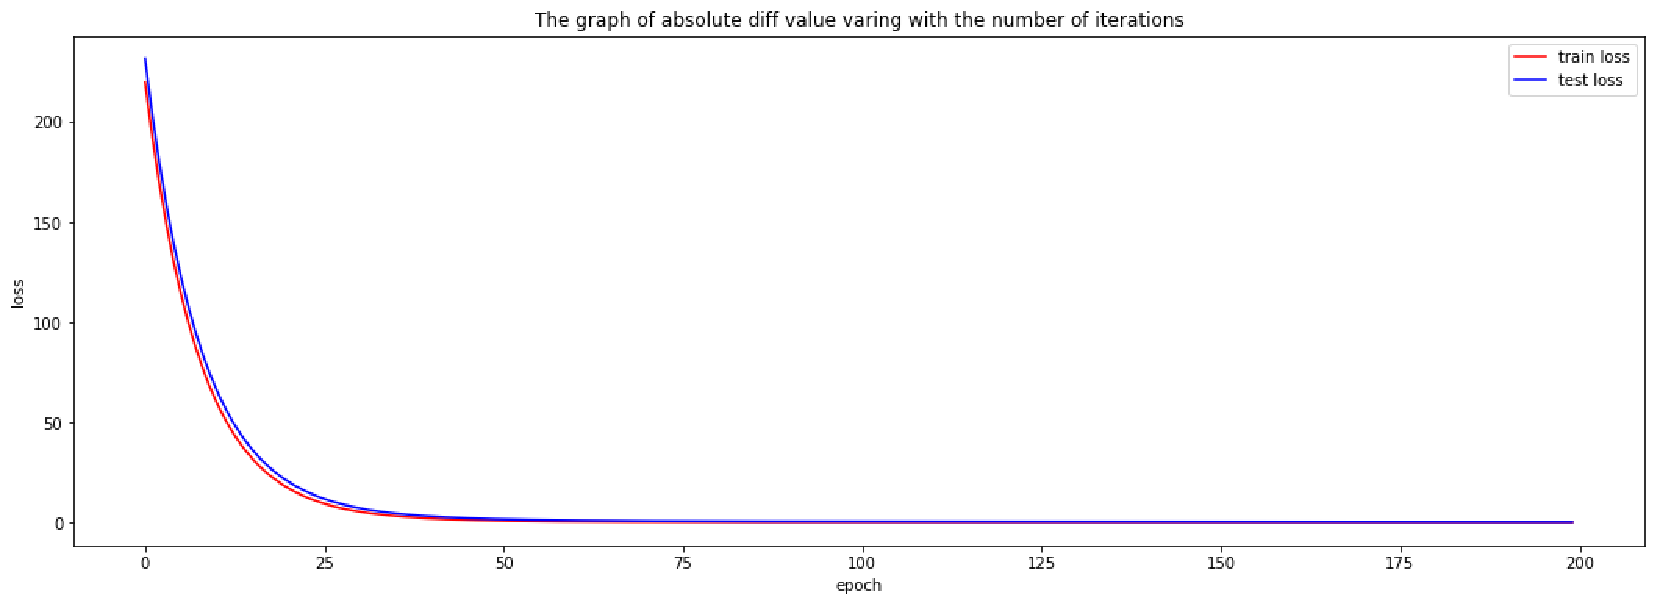
\includegraphics[width=\columnwidth]{lab1_loss}
		% Create a subtitle for the figure.
		\caption{Loss using gradient descent}
		% Define the label of the figure. It's good to use 'fig:title', so you know that the label belongs to a figure.
		\label{fig:tf_plot}
		\end{center}
	\end{figure}

\section{Conclusion}
	Through this experiment,I have experience solving a linear regression problem of a small scale dataset as well as the process of optimization and adjusting parameters.Also,I get the loss under closed-form solution and stochastic gradient descent and compare them(see TABLE III).It is apparent that closed-form solution for regression problem is precise but stochastic gradient descent is also a good method to handle the task.
\begin{table}[!hbt]
		% Center the table
		\begin{center}
		% Title of the table
		\caption{Comparison}
		\label{tab:simParameters}
		% Table itself: here we have two columns which are centered and have lines to the left, right and in the middle: |c|c|
		\begin{tabular}{|c|c|c|}
			% To create a horizontal line, type \hline
			\hline
			Loss & training set & validation set\\
			\hline
			initial Loss & 219.67849370889007 & 231.59647054171768\\
			\hline
			closed-form &  5.19398968642731e-19 &  0.02691910042021025\\
			\hline
			gradient descent & 0.10066842602334752 &  0.21471788009638246\\
			\hline
		\end{tabular}
		\end{center}
	\end{table}



% Your document ends here!
\end{document}